\documentclass[suppldata]{interact}
\usepackage[T1]{fontenc}
\usepackage[utf8]{inputenc}
\usepackage{amsmath,amssymb,amsthm}
\usepackage{graphicx,booktabs,array,longtable,placeins,xurl}
\usepackage{xcolor,hyperref,caption}
\usepackage[authoryear,sort]{natbib}
\bibpunct[, ]{(}{)}{;}{a}{,}{,}
\usepackage[mathlines]{lineno}
\usepackage{setspace}
\doublespacing
\renewcommand\linenumberfont{\normalfont\scriptsize\sffamily}
\setlength\linenumbersep{10pt}
\setlength{\emergencystretch}{2em}
\providecommand{\tablebodyfont}{\small}
\providecommand{\tablefootnotefont}{\small}
\newtheorem{proposition}{Proposition}[section]
\newtheorem{corollary}[proposition]{Corollary}
\hypersetup{hidelinks}
\raggedbottom
\begin{document}
\articletype{RESEARCH ARTICLE}
\title{When Do Extreme-Demand Models Improve Tariff Decisions? A Computational Comparison}
\author{\name{Mingyu Huang\textsuperscript{a}\thanks{CONTACT Mingyu Huang. Department of Statistics and Data Science, School of Mathematics and Statistics, Yunnan University, Chenggong Campus, South Section of East Outer Ring Road, Chenggong District, Kunming, Yunnan 650500, China. Email: huangmingyu@stu.ynu.edu.cn}, Jiangweixi Wang\textsuperscript{a}, Zheng Gao\textsuperscript{a}, Yihang Yuan\textsuperscript{a}, and Zhengjun Yang\textsuperscript{b}}
\affil{\textsuperscript{a}Department of Statistics and Data Science, School of Mathematics and Statistics, Yunnan University, Kunming 650500, China; \textsuperscript{b}Department of Mathematics, School of Mathematics and Statistics, Yunnan University, Kunming 650500, China}}
\maketitle
\noindent\textbf{Short title:} Extreme-Demand Tariff Decisions
\begin{abstract}
Forecast comparisons for extreme demand can reverse after a predictive distribution enters a tariff decision. We develop a paired computational framework linking distributional functionals to charging-mode selection, contract choice, and full-action regret. A constrained Expected Shortfall representation characterizes contract demand, while pair-specific Wasserstein bounds quantify the stability of optimized tariff contrasts. Across 10,000 histories, GEV-minus-KDE mean regret is +0.822, -3.887, +5.470 thousand CNY/month in the actual-demand, contract-demand, and capacity regions, respectively, although both methods use the same monthly maxima. Four-fold held-out CRPS selects the TAIL threshold, and simultaneous history-level intervals quantify focal regret contrasts. Rolling forecasts from eight manufacturing facilities illustrate how the evaluation is applied to observed load and illustrative tariff charges.
\end{abstract}
\begin{keywords}
Monte Carlo comparison; extreme-value estimation; probabilistic forecasting; decision loss; electricity demand tariffs
\end{keywords}
\linenumbers
\section{Introduction}
\label{sec:introduction}

Industrial electricity tariffs can make a plant's monthly peak demand
as important as its total energy use. Under capacity subscriptions and
contract-demand schemes, customers choose a tariff mode or contract
level before the future peak is known, so the predictive distribution
of maximum demand affects both the selected action and its expected
cost \citep{BjarghovEtAl2022,WuEtAl2022,LimaEtAl2026,SungKwon2026}.
The economic value of a peak-demand forecast depends on how it enters
the tariff decision. The central question is which features of the predictive
distribution matter for that decision and how errors in those features
translate into economic loss.

Research relevant to this question has developed along three
complementary lines. Contracting and capacity-subscription studies
optimize subscribed or contracted demand under uncertain load and
examine the sensitivity of contract choices to demand and price errors
\citep{BjarghovEtAl2022,WuEtAl2022,FerdavaniEtAl2018,FerdavaniHooshmand2019,LimaEtAl2026}.
Probabilistic-forecasting research places predictive distributions
inside downstream operational problems, including reserve planning,
market bidding and scheduling, and decision-focused forecast
combination
\citep{WangEtAl2023,BeykirchEtAl2024,StratigakosEtAl2025}.
More broadly, predict-then-optimize and decision-focused learning
connect predictive models directly to downstream optimization
objectives
\citep{ElmachtoubGrigas2022,MandiEtAl2024}.
A related application-driven literature evaluates forecasts through
their operational or economic consequences and shows that statistical
and decision-based rankings can differ
\citep{MaciejowskaEtAl2026,HoubenEtAl2026}.
Together, these studies connect forecast quality, tariff design, and
downstream cost.

Extreme-value comparisons between block maxima and peaks over threshold
depend on the generating mechanism, dependence, and statistical target
\citep{BuecherZhou2021}. Threshold selection balances approximation
and estimation uncertainty \citep{ScarrottMacDonald2012}. Here the
evaluation target is the action induced by a tariff with a discrete
mode choice and a continuous contract level.

For competing industrial tariffs, a useful analysis follows one
predictive distribution through the complete decision. Capacity
charging is distribution-independent, actual-demand charging depends
on the mean, and contract-demand charging depends on an optimized
exceedance cost. The tariff choice therefore compares three mode values
that respond differently to the same predictive error. The analysis
must distinguish errors that change the tariff mode from errors that
change the contract level within contract demand, while retaining the
common distributional perturbation across competing costs.

The statistical contribution is to track common forecast error through
optimized tariff-cost contrasts and the complete action. This shows
when shared error cancels in mode selection and when the remaining
functional error changes contract choice or regret.

We construct a controlled comparison of distribution estimators under a
mixed tariff action. The experiment pairs fitted predictive laws within
each demand history, fixes the tariff cells before method comparison,
and evaluates both distributional functionals and the complete action
under an analytic oracle. The tariff representation identifies the
mean, stop-loss curve, and constrained Expected Shortfall as the
functionals that control the action; exact regret decomposition and
contrast-specific Wasserstein margins explain why estimator rankings
change across tariff regions. We test those rankings across
alternative demand mechanisms, sample lengths, and rolling forecasts
from manufacturing-load data.

\section{Tariff decision framework}
\label{sec:tariff-decision-framework}

Let $M\geq0$ be the next monthly maximum with predictive law $F$, finite
mean $\mu_F$, and stop-loss transform
$H_F(t)=\mathbb{E}_F[(M-t)_+]=\int_t^\infty[1-F(x)]\,dx$.
The capacity, actual-demand, and contract-demand costs are, respectively,
\begin{equation}
\label{eq:tariff-costs-cssc}
C_F(\mathrm{cap})=r_cS,\quad
C_F(\mathrm{act})=r_d\mu_F,\quad
C_F(\mathrm{con},D)=r_d\{D+\kappa H_F(\alpha D)\},
\quad D\in[\delta S,S].
\end{equation}
Here $S$ is reference capacity, $r_c$ and $r_d$ are rates,
$\alpha$ is the overage threshold multiplier, and $\kappa$ is
the penalty multiplier. Thus tariff decisions depend on the mean and
the stop-loss curve, rather than on a tail quantile alone
(Equation~\eqref{eq:tariff-costs-cssc}).

\subsection{Contract optimization and action regret}
\label{sec:contract-optimization}
The contract objective is convex. For an interior optimum when
$\kappa\alpha>1$, its threshold $\alpha D^*$ is a generalized quantile
at $p^*=1-(\kappa\alpha)^{-1}$, constrained to
$[\alpha\delta S,\alpha S]$. Equivalently, optimizing contract
demand amounts to minimizing a constrained Expected Shortfall
representation \citep{RockafellarUryasev2002}:
\begin{equation}
\label{eq:contract-constrained-es}
V_F(\mathrm{con})=
\frac{r_d}{\alpha}
\min_{t\in[\alpha\delta S,\alpha S]}
\left\{t+\frac{H_F(t)}{1-p^*}\right\}.
\end{equation}
The other optimized mode costs are $V_F(\mathrm{cap})=r_cS$ and
$V_F(\mathrm{act})=r_d\mu_F$. The oracle chooses the smallest of these
three values. For a fitted law $\widehat F$, define its selected
mode and contract level by the same optimization. Its oracle regret is
$R_F(\widehat a)=C_F(\widehat a)-V_F^*$, where
$V_F^*=\min_m V_F(m)$. If $\widehat m$ is contract demand, regret
contains both any cost of selecting the wrong mode and error in the
contract level:
\begin{equation}
\label{eq:within-contract-loss}
R_F(\widehat a)=
\{V_F(\widehat m)-V_F^*\}
+\{C_F(\widehat a)-V_F(\widehat m)\}.
\end{equation}
The second term is zero for the capacity and actual-demand modes.
These two components are computed for every simulated action.

\subsection{Decision stability}
For two laws $F,G$ with finite first moments, write
$W_1(F,G)=\int_0^\infty|F(x)-G(x)|\,dx$ for their one-dimensional
Wasserstein distance. The primitive-action envelope is
\begin{equation}
\label{eq:epsilon}
\varepsilon(F,G)=
\max\!\left\{r_d|\mu_F-\mu_G|,
r_d\kappa\sup_{D\in[\delta S,S]}
|H_F(\alpha D)-H_G(\alpha D)|\right\}.
\end{equation}
For an exact minimizer $\widehat a$ under $G=\widehat F$,
$R_F(\widehat a)\leq2\varepsilon(F,G)$; the guarantee does not
apply to an arbitrary action. If $F$ has a unique optimal mode with
gap $\gamma_F$, $2\varepsilon(F,G)<\gamma_F$ preserves that mode.
The envelope bounds mode values separately and can count common
forecast perturbations twice. A tariff-contrast bound retains their
cancellation.

\begin{proposition}[Tariff-contrast stability]
\label{prop:contrast-wasserstein-cssc}
Let $V_F(m)$ be the optimized mode values of
Equation~\eqref{eq:tariff-costs-cssc}, with a common feasible contract
set and $r_d,\kappa,\alpha>0$. For every distinct pair of modes
$m,n\in\{\mathrm{cap},\mathrm{act},\mathrm{con}\}$,
\[
|[V_F(m)-V_F(n)]-[V_G(m)-V_G(n)]|
\leq K_{m,n}W_1(F,G),
\]
where
\begin{equation}
\label{eq:contrast-constants-cssc}
K_{\mathrm{cap},\mathrm{act}}=r_d,\quad
K_{\mathrm{cap},\mathrm{con}}=r_d\kappa,\quad
K_{\mathrm{act},\mathrm{con}}
=r_d\max\{1,|1-\kappa|\}.
\end{equation}
If $m_F^*$ is unique, put
$\gamma_{F,m}=V_F(m)-V_F(m_F^*)>0$ for each competitor.
The mode selected under $G$ equals $m_F^*$ whenever
\begin{equation}
\label{eq:contrast-radius-cssc}
W_1(F,G)<\rho_F^{\mathrm{contrast}}
=\min_{m\ne m_F^*}\frac{\gamma_{F,m}}{K_{m,m_F^*}}.
\end{equation}
\end{proposition}
For capacity versus actual demand, the contrast is the expectation
of $r_cS-r_dM$, whose Lipschitz coefficient is $r_d$.
For capacity versus contract demand, it is the supremum over feasible
$D$ of the expectation of
$r_cS-r_dD-r_d\kappa(M-\alpha D)_+$; each integrand has coefficient
$r_d\kappa$. For actual versus contract demand, write
$g_D(x)=x-D-\kappa(x-\alpha D)_+$.
Then $[V_F(\mathrm{act})-V_F(\mathrm{con})]/r_d
=\sup_D\mathbb E_F[g_D(M)]$. The slopes of $g_D$ are $1$ and
$1-\kappa$, giving coefficient
$r_d\max\{1,|1-\kappa|\}$. Applying the
Kantorovich--Rubinstein inequality before the supremum gives the
three bounds \citep{RachevRomisch2002}. The direct actual--contract
coefficient improves the sum of separate mode coefficients by the
factor $(1+\kappa)/\max\{1,|1-\kappa|\}$, equal to three at
$\kappa=2$. Appendix~S1 gives the full proof.

\begin{corollary}[Full-action regret]
For nonnegative laws $F,G$ with finite first moments, if
$\widehat a_G$ exactly minimizes the tariff cost under $G$, then
\[
R_F(\widehat a_G)\leq r_d\max\{1,\kappa\}W_1(F,G).
\]
\end{corollary}
Each realized primitive-action cost is nondecreasing in demand and
has slope between $0$ and $L=r_d\max\{1,\kappa\}$. The cost difference
between any two actions is therefore $L$-Lipschitz. If $a_F$ is
optimal under $F$, optimality of $\widehat a_G$ under $G$ gives
$\mathbb E_G[c(M,\widehat a_G)-c(M,a_F)]\leq0$; applying the
Kantorovich--Rubinstein inequality to this action contrast proves
the bound. A fitted-action optimization gap at most $\zeta$ adds
$\zeta$ to the right-hand side.
The radii have demand units (kW here). For the primary tariff
$\kappa=2$, the actual--contract constant is $r_d$, compared with
$r_d(1+\kappa)=3r_d$ from separate mode bounds. The resulting
numerical certificates are evaluated on the same decision rows in
Section~\ref{sec:results-stability}.

\section{Distribution estimation and tariff actions}
\label{sec:distribution-estimation-actions}

\subsection{Distribution estimators}
\label{sec:distribution-estimators}

We compare five predictive constructions, grouped by the information
used to estimate the monthly-maximum distribution. TAIL and EVENT-EMP
use the same event-level history, whereas GEV, KDE, and EMP use the
same 24 monthly maxima. Comparisons within these two groups therefore
separate distributional construction from information source;
comparisons across groups evaluate complete forecasting procedures.

TAIL models event-level exceedances above candidate empirical
threshold quantiles
\[
0.90,\quad 0.925,\quad 0.95,\quad 0.975.
\]
For each 24-month history, threshold selection uses four disjoint
month-level validation folds. Each fold fits on 18 months and scores the
remaining six monthly maxima by CRPS; the candidate with the smallest
mean score across all 24 validation outcomes is selected. Excesses above a candidate
threshold follow a generalized Pareto model \citep{DavisonSmith1990},
while monthly exceedance counts are represented by a Poisson or
negative-binomial distribution according to the observed count
dispersion. Candidate specifications are compared by deterministic held-out
CRPS, with a minimum-exceedance screen and a finite-mean GPD requirement.
The selected full-history fit receives a 500-resample shape-interval
diagnostic and an observed-support check.

After selection, we retain the selected threshold quantile, recompute
its numerical value using all 24 months, and refit the excess law,
count model, and subthreshold component at that threshold. The resulting monthly-maximum law combines the empirical
distribution of monthly subthreshold maxima with the fitted
exceedance-count and excess distributions. It is required to have a
finite first moment and support compatible with the observed event
history. When the primary tail
specification is unavailable, the prespecified fallback sequence uses
an exponential tail and then the empirical monthly-maxima distribution.
Appendix~S1.3 details the screening thresholds, selection score,
and fallback rules.

EVENT-EMP provides a nonparametric event-level construction from the
same 24-month event history. Let $\widehat G_E$ denote the pooled
empirical distribution function of event-level maxima and let $N_m$
denote the observed total number of events in month $m$. Conditional on
$N_m$, the induced monthly-maximum distribution has CDF
$\widehat G_E(x)^{N_m}$. Averaging over the empirical distribution of
monthly event counts yields
\[
\widehat F_{\mathrm{EE}}(x)
=
\frac{1}{24}
\sum_{m=1}^{24}
\widehat G_E(x)^{N_m}.
\]
EVENT-EMP therefore propagates the empirical event-value and monthly
event-count distributions directly to monthly maximum demand. Together
with TAIL, it provides an event-level reference for examining how
different distributional constructions translate the same underlying
event history into tariff-relevant predictive laws.

The three monthly-maxima constructions use the 24 observed monthly
maxima. GEV fits a generalized extreme-value distribution
\citep{Coles2001} using sample
probability-weighted moments to construct the first three L-moments
\citep{Hosking1990}, from which the distribution parameters are
obtained deterministically. The shape search is restricted to a
prespecified interval contained within the finite-mean region. For
numerical evaluation, the fitted law is conditioned on the
nonnegative portion of its natural support. Fits failing the parameter or
support checks revert to the empirical monthly-maxima distribution.

KDE is fitted to the 24 observed monthly maxima using a Gaussian kernel with bandwidth
\[
h=1.06\,s\,n^{-1/5},
\]
where $s$ is the sample standard deviation and $n$ the number of
monthly maxima. The equal-weight Gaussian mixture is conditioned on
nonnegative support. A numerically degenerate training sample triggers
an empirical fallback.

EMP assigns equal mass to the observed monthly maxima.

\subsection{From estimated distributions to tariff actions and regret}
\label{sec:estimated-actions-regret}

All five fitted predictive distributions enter the tariff-action map
of Section~\ref{sec:tariff-decision-framework} through deterministic
evaluation of their means, stop-loss transforms, and quantiles. EMP and
EVENT-EMP use exact finite sums, KDE uses truncated-normal expressions,
and GEV and TAIL use deterministic inversion and integration where
required. The primary TAIL threshold is selected by deterministic held-out
CRPS. Predictive simulation does not enter the final tariff functionals
or regret calculations.

Each fitted law is then evaluated over the continuous feasible interval
$\mathcal D_S=[\delta S,S]$ using the contract objective in
Section~\ref{sec:contract-optimization}. The convex objective is
minimized from its boundary and generalized-quantile conditions, using
exact adjacent support points for discrete laws and deterministic root
finding for continuous laws. We resolve exact tariff-mode ties and nonunique discrete quantiles
using the prespecified deterministic conventions in Appendix~S1.4.

The selected tariff mode is
\[
\widehat m
\in
\operatorname*{arg\,min}_{m\in\mathcal M}
\widehat V(m).
\]
If $\widehat m=\mathrm{con}$, let $\widehat D$ denote the selected minimizing contract level and define
\[
\widehat a=a_{\mathrm{con}}(\widehat D).
\]
For $\widehat m=\mathrm{cap}$ or $\widehat m=\mathrm{act}$, the selected action is $a_{\mathrm{cap}}$ or $a_{\mathrm{act}}$, respectively, and $D$ has no economic role in that action. Oracle functionals and actions are evaluated directly from the analytic data-generating distribution by deterministic integration and inversion. Each tariff cell therefore has fixed oracle mode values, mode separation, and optimal action.

We distinguish two decision endpoints. In cells with a unique oracle
mode, tariff-mode correctness is the row-level indicator
$I(\widehat m=m_F^\ast)$, which evaluates only the discrete mode
choice. Oracle-mode accuracy denotes the percentage of correct mode selections across Monte Carlo replications within a scenario--method cell, reported as ``Acc.'' in the scenario tables. Economic performance is instead assessed through full-action regret under the true distribution,
\[
R_F(\widehat a)
=
C_F(\widehat a)-V_F^\ast.
\]
Under contract demand, this endpoint includes the cost of the selected contract level as well as the selected mode. Numerically, regret is recorded as
\[
\max\left\{0,\,
C_F(\widehat a)-V_F^\ast
\right\},
\]
where truncation at zero only guards against negative floating-point differences.

The comparison varies the predictive distribution while holding the
tariff decision rule fixed.

\section{Evaluation design and inference}
\label{sec:evaluation-design}
\label{sec:evaluation-inference}

\subsection{Controlled and stress experiments}
The primary experiment draws $10{,}000$ independent 24-month demand
histories from a Poisson--GPD event model. Each month has 200 bulk
events on $[45{,}000,80{,}000]$ kW, with scaled $\mathrm{Beta}(8,2)$
amplitudes, and $\mathrm{Poisson}(30)$ excess events above 80,000 kW
with GPD shape 0.15 and scale 12,000 kW. The monthly maximum is the
largest event. Specifically, $F_B$ is the CDF of
$45{,}000+35{,}000B$ for $B\sim\mathrm{Beta}(8,2)$, and $F_Z$
is the CDF of $80{,}000+Y$ for
$Y\sim\mathrm{GPD}(0.15,12{,}000)$. An analytic oracle gives
the monthly-maximum CDF,
$F_M(x)=F_B(x)^{200}\exp\{30(F_Z(x)-1)\}$, mean, stop-loss, and
optimal tariff action.

TAIL, EVENT-EMP, GEV, KDE, and EMP are fitted to the same history
and evaluated in nine fixed tariff cells: $(\alpha,u)=(1.05,0.620),
(1.05,0.630)$ and $\alpha=1.20$ with
$u\in\{0.400,0.450,0.455,0.625,0.630,0.635,0.700\}$,
where $u=\mu_F/S$. We use $r_d=36$, $r_c=22.5$ CNY/(kW month),
$\kappa=2$, and $\delta=0.40$. The cells span three oracle mode
regions and gaps of different sizes; they were fixed from oracle
geometry before method comparison. The rates are illustrative coefficients for the computational design.
The crossed-grid analysis reuses
1,000 histories over four $\alpha$ values and 19 utilization levels.
Additional designs raise the interior contract quantile target to
$0.90$, $0.95$, and $0.99$, change Poisson--GPD events to
negative-binomial counts with Weibull excesses, vary event clustering
and training length, and vary fitted support. Parameters and complete
results appear in Appendix~S1.

\subsection{Endpoints and inference}
\label{sec:controlled-mechanism}
Distributional endpoints are relative errors in the mean and
tariff-specific stop-loss, with $q_{0.99}$ error as a conventional
upper-tail comparator. Decision endpoints are mode correctness and
full-action regret, both absolute and divided by the oracle cost.
Regret is evaluated under the analytic oracle after each fitted law
has selected its action. Within each history, the nine cells are
equally weighted within their oracle-mode region; methods are paired
on history. Reported regional contrasts use paired Student $t$
95\% intervals over the 10,000 independent histories. Six focal
matched-information comparisons also use simultaneous history-level
max-$|T|$ intervals based on 5,000 bootstrap resamples (Table~S18). Within-method Spearman correlations between absolute relative
distributional errors and regret use history-level averages;
ten correlation contrasts receive centered, studentized max-$|T|$
familywise intervals from 2,000 paired history bootstraps. Numerical
optimizer checks are in Appendix~S1.15.

\subsection{External manufacturing-load analysis}
\label{sec:external-manufacturing}
The external experiment uses public one-minute load records from
10 South Korean factories, March--September 2019
\citep{Lee2022KoreanFactories,LeeFigshareV9}. We reconstruct complete
15-minute averages, remove documented demand-response and 60-minute
rebound windows, and retain factory-months with at least 95\%
complete windows. Eight factories meet the fixed eligibility rule.
Four expanding-window origins forecast June--September monthly maxima.
The seven procedures are K-BLOCK (monthly block resampling), K-EMP
(empirical maxima), K-GEV, K-GTAIL (validated event tail), K-KDE,
K-POINT (a point forecast), and K-UGPD (unconditional GPD).
They are compared by CRPS, upper-tail weighted CRPS, and 0.95/0.99
pinball loss. The implemented upper-tail score is twice the trapezoidal
integral of pinball loss $\rho_\tau(y-q_\tau)$ over
$\tau\in\{0.900,0.905,\ldots,0.995\}$; its fixed grid and
normalization are specified in Appendix~S1.13. All model selection
and normalization use training
months only. For origin $o$, let $s_o$ be the mean of its training
monthly maxima; the normalized reference capacity is $S_o(u)=1/u$,
or $s_o/u$ in kW. Predictive distributions select actions in the
nine illustrative tariff cells; each is scored by the hypothetical
next-month charge divided by $s_o$. Methods share the same scale and
tariff within each factory-origin. The next-month observation is used
only for scoring, never for setting $S_o$.
Four origin differences are averaged within factory, then paired
$t$ intervals are constructed over eight factories. Processing,
validation, scoring, and fallback details are in Appendix~S1.13.

\section{Results}
\label{sec:results}

\subsection{Tariff geometry changes decision sensitivity}
\label{sec:results-geometry}

Oracle mode separation varies substantially across tariff
configurations. Panels (a) and (b) of
Figure~\ref{fig:tariff-geometry} show this structure for
$\alpha=1.20$: as utilization increases, the optimal tariff moves
from actual demand to contract demand and then to capacity charging. Across the nine primary cells, the relative oracle gap ranges
from $0.093\%$ to $10.732\%$. The smallest gaps occur close to
mode transitions, while more separated cells provide larger margins
before the preferred tariff can change (Table~S12).

This variation in tariff geometry is reflected in decision performance.
Figure~\ref{fig:tariff-geometry}(c,d) shows that both full-action regret
and oracle-mode accuracy vary substantially across tariff cells, even
though the same fitted predictive distribution is reused within each
history. The tariff therefore changes how a given distributional error
is translated into an economic decision.

\begin{figure}[!htbp]
\centering
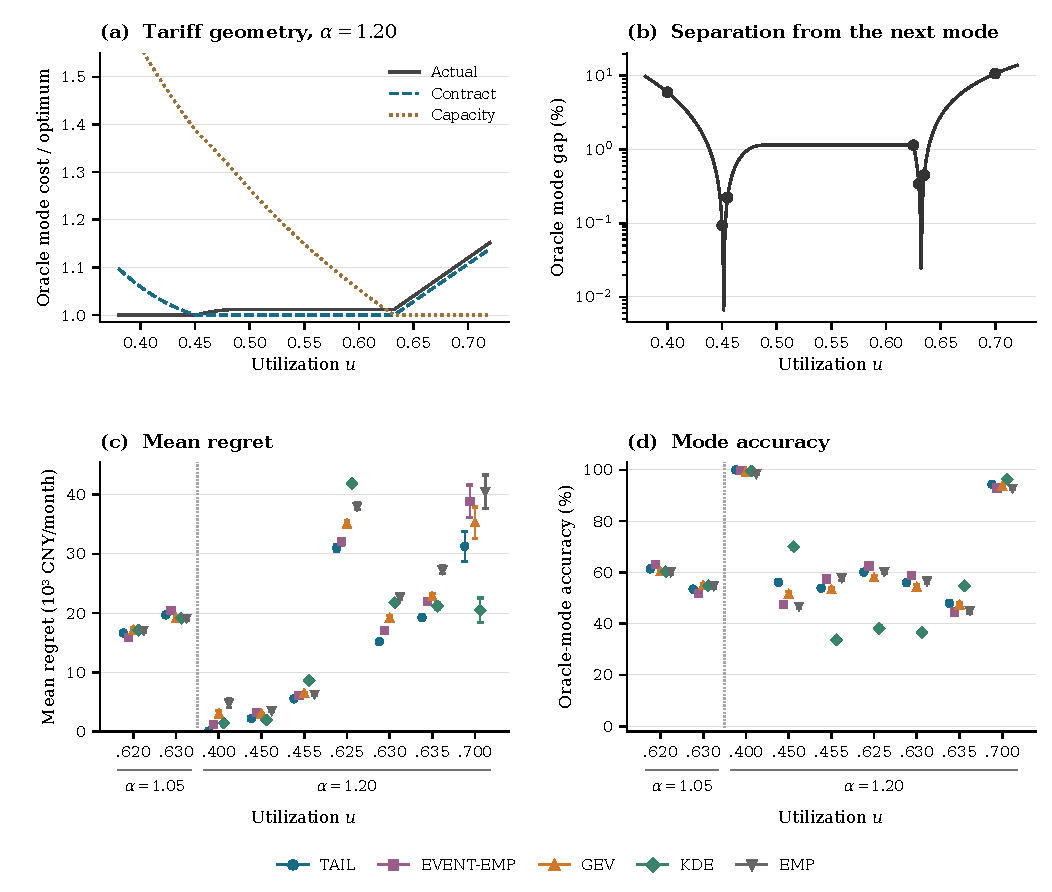
\includegraphics[width=\linewidth,height=0.65\textheight,keepaspectratio]{figures/Figure_1.pdf}
\caption{\textbf{Tariff geometry and primary decision performance.}
\textbf{(a)} Optimized oracle mode costs relative to the minimum and
\textbf{(b)} the relative separation between the two lowest mode values
for $\alpha=1.20$; dots in (b) mark the seven primary cells in this
block.
\textbf{(c)} Mean full-action regret with pointwise Student $t$
95\% intervals.
\textbf{(d)} Oracle-mode accuracy with Wilson 95\% intervals across
all nine primary tariff cells. Each method--cell summary uses
10,000 independent histories. The lower panels use equally spaced
positions for the prespecified cells; labels give utilization $u$ and
$\alpha$.}
\label{fig:tariff-geometry}
\end{figure}

\subsection{Economic rankings change with tariff geometry}
\label{sec:results-economic-value}

The identical $q_{0.99}$ errors of EVENT-EMP and EMP in
Figure~\ref{fig:statistical-regret}(a) are structural: with only
24 monthly maxima, EMP's empirical 0.99 quantile is the largest
observed maximum; EVENT-EMP also reaches the largest observed
event maximum at that probability. The archived 90,000 paired
method--history--cell rows agree exactly on $q_{0.99}$, while
their selected tariff modes agree in 82,513 rows (91.68\%).
Their decision functionals and actions therefore remain distinct.

Forecast accuracy and economic performance ranked the methods
differently. TAIL had the smallest median absolute relative $q_{0.99}$
error, while the lowest-regret method varied by tariff region
(Table~S17;
Figure~\ref{fig:statistical-regret}(a)). Across all five predictive
methods, regret was more strongly associated with errors in the mean
and stop-loss functional than with $q_{0.99}$ error; all ten
simultaneous intervals for these correlation differences were positive
(Table~S7).

Methods using the same information can have different regional regret.
GEV-minus-KDE mean-regret contrasts were $+0.822$, $-3.887$, and $+5.470$ thousand CNY/month in the actual-demand,
contract-demand, and capacity regions. Their simultaneous 95\%
intervals were $[+0.624, +1.020]$; $[-4.236, -3.539]$; and $[+4.658, +6.283]$ (Table~S18). The normalized
mean differences were $+0.015$; $-0.074$; and $+0.114$ percentage points of oracle cost.
TAIL-minus-EVENT-EMP contrasts
were $-0.481$, $-1.160$, and $-3.643$ thousand CNY/month in those regions. The paired
intervals are reported in Table~S11.

A matched event-level comparison holds TAIL's selected threshold,
count law, and subthreshold component fixed while replacing its GPD
excess distribution with the empirical excess law. Across 10,000
histories per setting, the GPD excess fit reduced nine-cell mean regret
by $1.911$ thousand CNY/month (95\% paired interval
$[1.681,2.141]$) under Poisson--GPD and by $2.060$
($[1.807,2.313]$) under negative-binomial--Weibull. Under the
negative-binomial--Weibull mechanism, the GPD-versus-empirical-excess
regret contrasts were $+3.597$ ($[+3.315,+3.879]$) in the
actual-demand region, $-4.694$ ($[-5.096,-4.292]$) in the
contract-demand region, and $-1.132$ ($[-1.481,-0.783]$) in the
capacity region (Table~S15). Thus, the decision value of GPD tail
extrapolation varied with the tariff region even under a common event
history and count model.

The complete-procedure TAIL--KDE comparison uses different information
resolutions and likewise depends on tariff geometry. TAIL has lower
regional mean regret in the actual-demand
and contract-demand regions but higher mean regret in the capacity
region. The capacity average masks substantial variation across its
three cells: the TAIL--KDE contrast changes sign and reaches
$+12.945$ thousand CNY/month at
$(\alpha,u)=(1.20,0.700)$. At this cell, departures from the oracle capacity mode incur
mode-selection loss; any additional within-mode loss depends on the
mode selected. Table~\ref{tab:table_3} reports method-specific
regional regret and oracle-mode accuracy.

The same pattern extends beyond the nine primary cells.
Figure~\ref{fig:statistical-regret}(e--h) shows that both
TAIL--KDE and GEV--KDE contrasts vary with utilization and oracle mode
across the 76-cell crossed grid. Contract demand appears only in the
$\alpha=1.20$ block, while the other blocks contain actual-demand and
capacity regions. Complete five-method profiles are reported in
Figure~S8.

\begin{figure}[!htbp]
\centering
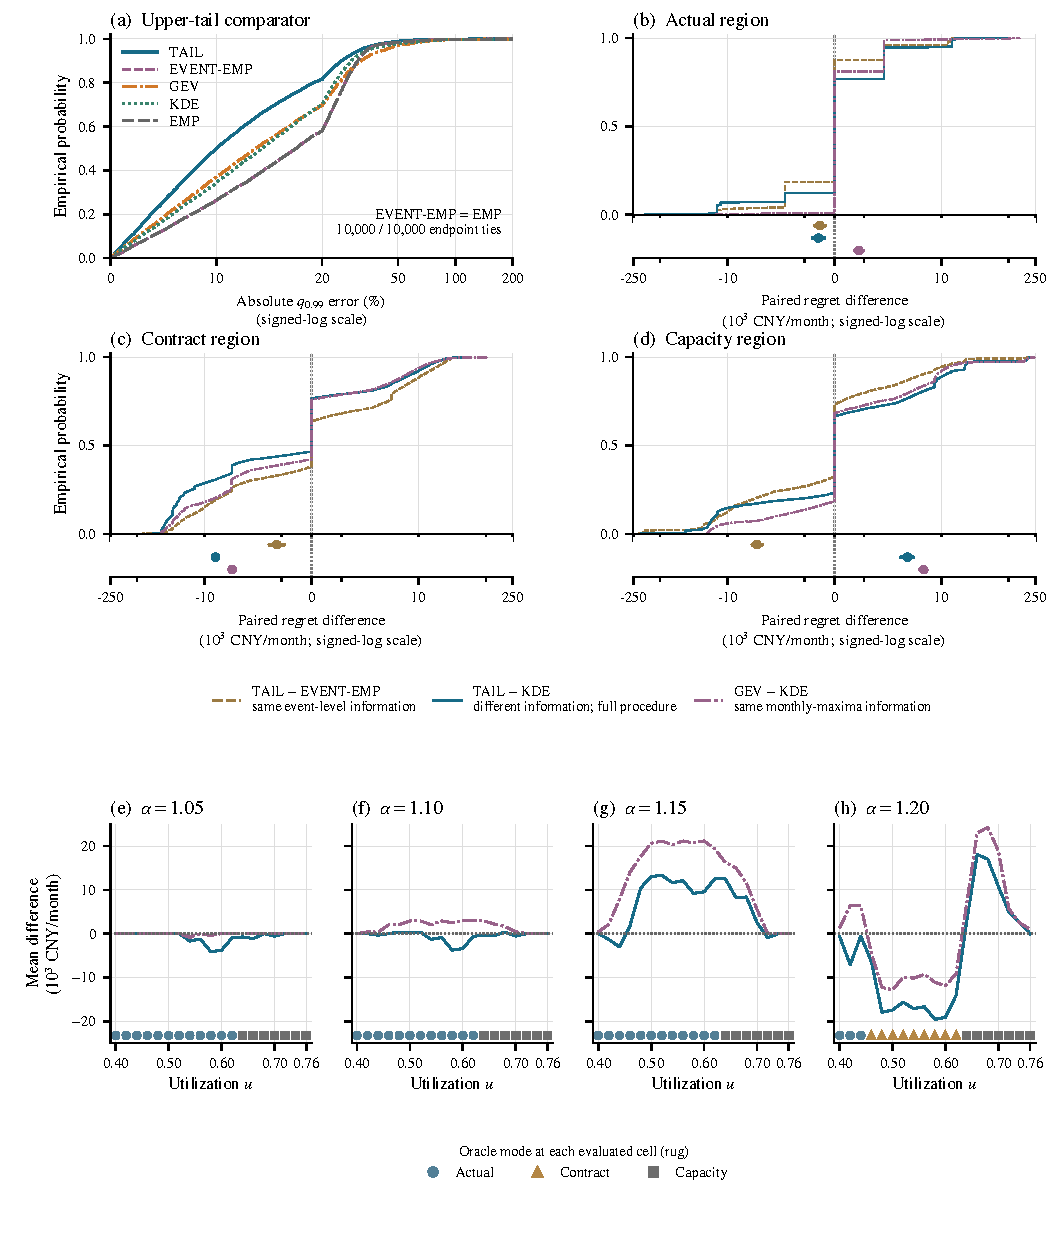
\includegraphics[width=\linewidth,height=0.65\textheight,keepaspectratio]{figures/Figure_2.pdf}
\caption{\textbf{Statistical fidelity and geometry-dependent economic
performance.}
\textbf{(a)} Empirical distributions of absolute relative
$q_{0.99}$ error over 10,000 histories per method; EVENT-EMP and EMP
coincide. The scale is linear up to $20\%$ and logarithmic beyond $20\%$.
\textbf{(b--d)} ECDFs of paired full-action-regret differences in the
actual-demand, contract-demand, and capacity regions after averaging
the three cells within each history. Negative values favour the first
named method; markers and bars show the mean difference and paired
Student $t$ 95\% interval.
\textbf{(e--h)} Mean-regret contrasts for TAIL--KDE and GEV--KDE
across the 76-cell crossed tariff grid, using 1,000 histories per
method--cell; rugs indicate the oracle mode at each evaluated cell. TAIL--EVENT-EMP compares methods using the
same event-level information, whereas GEV--KDE compares methods using
the same monthly-maxima information.}
\label{fig:statistical-regret}
\end{figure}

\subsection{Tariff contrasts sharpen demand-scale stability}
\label{sec:results-stability}

Define $d_{MV}=2\max_m|V_{\widehat F}(m)-V_F(m)|/\gamma_F$,
where $\gamma_F$ is the best-to-second-best oracle mode gap.
The competitor-specific mode-value condition held more often than the
scalar $d_{MV}<1$ condition because it retains the gap and estimation
error associated with each competing mode separately
(Figure~\ref{fig:mode-stability}(a,b)). No observed tariff-mode errors occurred among decisions satisfying
either condition.

The same ordering appears on the demand scale. The contrast-aware
Wasserstein radius was never smaller than the mode-wise pairwise radius
and was strictly larger in four of the nine primary tariff cells
(Table~S12). It was three times larger in three cells where
actual demand and contract demand formed the limiting comparison, and
1.5 times larger in one cell where tightening that comparison caused
capacity to become the limiting competitor. Using upper endpoints of
the combined numerical $W_1$ brackets and the same solver
allowance, the contrast-Wasserstein check passed for $59{,}410/450{,}000$
decisions ($13.202\%$), versus $27{,}352$ ($6.078\%$) for the
mode-wise pairwise check. The full-action regret check
$LW_{1,\rm upper}+\zeta_{\rm full,num}<\gamma_F$ passed for
$31{,}677$ ($7.039\%$). No observed mode-selection errors occurred
among passing rows. These numerical check pass rates use the known
generating law in simulation (Tables~S13--S14; Figure~S3).

Mode preservation does not by itself determine the full tariff action.
Actual-demand and capacity modes have no remaining within-mode choice,
so a correct selection of either mode gives zero within-mode excess.
Contract demand retains the continuous choice of contract level, and
positive within-contract regret can therefore remain after the tariff
mode has been selected correctly
(Figure~\ref{fig:mode-stability}(c,d)).

\begin{figure}[!htbp]
\centering
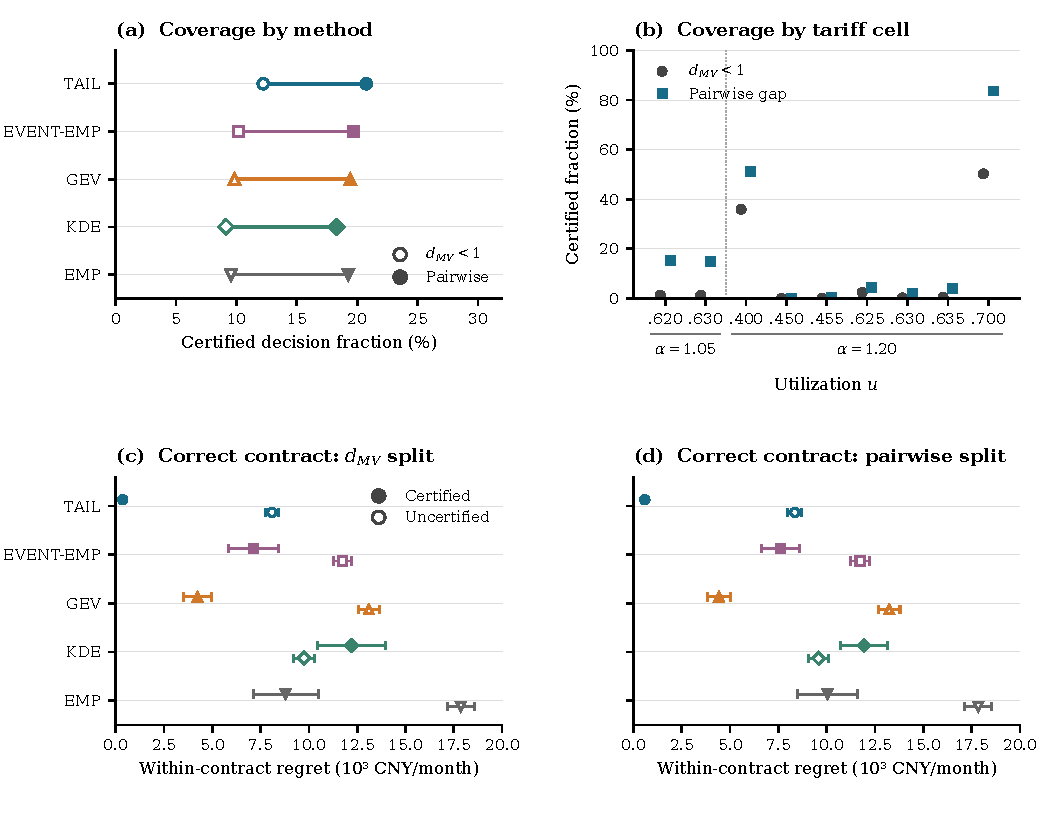
\includegraphics[width=\linewidth,height=0.65\textheight,keepaspectratio]{figures/Figure_3.pdf}
\caption{\textbf{Mode stability and residual within-contract regret.}
\textbf{(a,b)} Fractions of primary decisions satisfying the scalar
$d_{MV}<1$ and competitor-specific mode-value sufficient conditions,
by predictive method and tariff cell.
\textbf{(c,d)} Mean within-contract regret among decisions for which
contract demand is both oracle optimal and selected, split according
to whether the corresponding stability condition is satisfied.
Markers and bars show means and pointwise Student $t$ 95\% intervals
across eligible histories. Actual-demand and capacity decisions are
absent from (c,d) because their within-mode excess is zero once the
mode is fixed.}
\label{fig:mode-stability}
\end{figure}

\subsection{Stress designs reveal mechanism-dependent rankings}
\label{sec:results-stress}

The negative-binomial--Weibull challenge compares the same five
fitting procedures under a different joint count and severity
mechanism (Figure~S7; Tables~S4--S5). Across the actual-demand,
contract-demand, and capacity regions, TAIL-minus-EVENT-EMP
mean-regret contrasts were $-29.85$, $-12.37$, $+7.81$ thousand CNY/month. The corresponding GEV-minus-KDE
contrasts were $+5.06$, $-34.32$, $+1.98$ thousand CNY/month. Table~S5 reports paired intervals.

Changing $p^*$ changes the penalty multiplier and the
oracle-region composition. On four utilization cells that
remain contract optimal at all three targets, GEV-minus-KDE
paired mean regret differences are $-1.057$, $+13.813$, and
$-1.368$ thousand CNY/month at $p^*=0.90$, $0.95$, and $0.99$.
At $0.99$, the paired interval is $[-3.099,+0.363]$.
TAIL-minus-EVENT-EMP differences are $-8.165$, $-15.511$,
and $-71.392$ in the same order (Table~S16).

Parameter-recovery, threshold-fixed bootstrap, and physical-clipping
results are reported in the Supporting Information.

\subsection{External rankings depend on the predictive target}
\label{sec:results-external}

Across the eight factories, point estimates favour K-BLOCK and
K-KDE for whole-distribution CRPS, whereas K-GTAIL has lower
upper-tail weighted scores and $q_{0.99}$ pinball loss than these
two methods. The corresponding factory-paired intervals include
zero (Table~S9). K-GTAIL's final specification passed its fitting
gates in 15 of 32 factory--origin cases, with 13 exponential-tail
and four empirical fallbacks; K-GEV passed in eight cases and used
its empirical fallback in the remaining 24 (Table~S8).

Figure~\ref{fig:korean-external}(e,f) compares normalized next-month
charges under the common illustrative tariff. Charge differences
vary by tariff cell for K-GTAIL versus K-BLOCK and the K-GEV pipeline
versus K-KDE
across the eight factories.

\begin{figure}[!htbp]
\centering
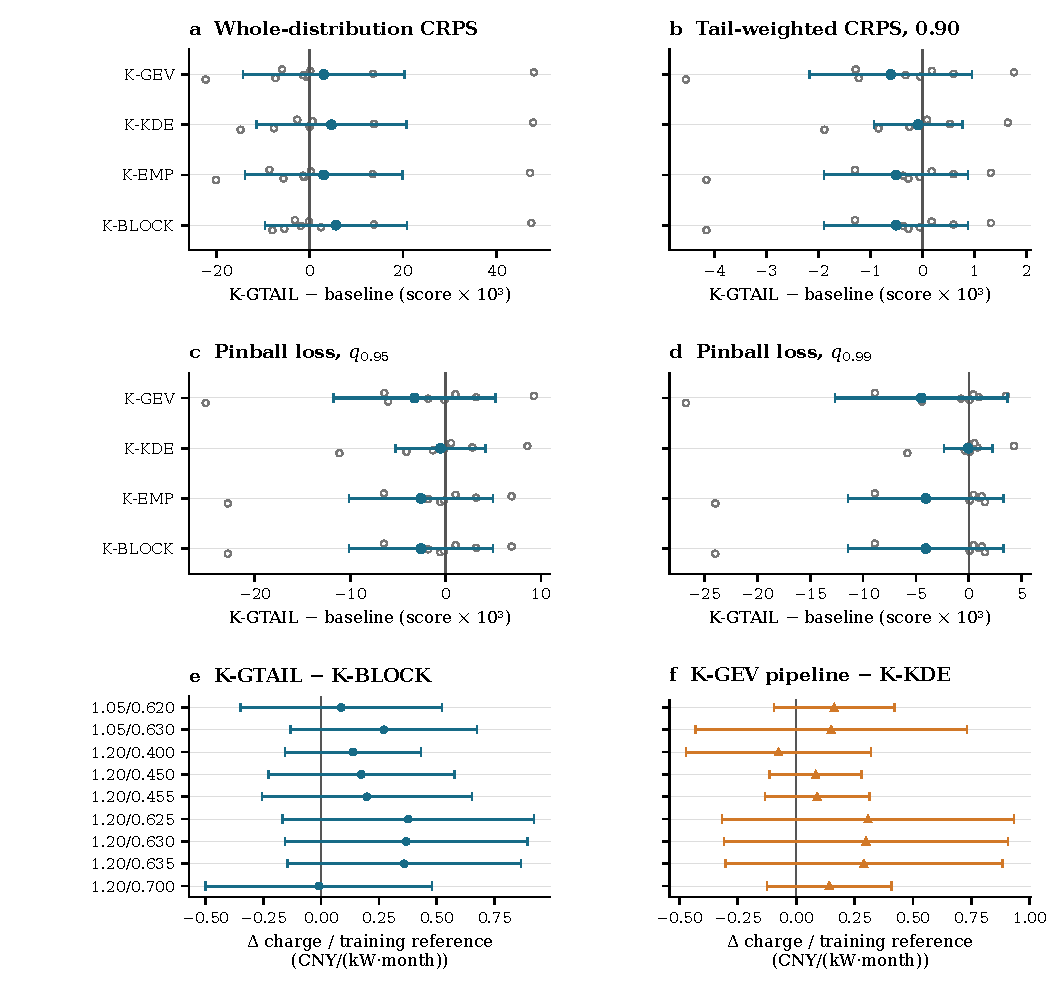
\includegraphics[width=\linewidth,height=0.65\textheight,keepaspectratio]{figures/Figure_4.pdf}
\caption{\textbf{External predictive and tariff-linked comparisons.}
The analysis uses eight manufacturing facilities with four rolling
forecast origins per facility.
\textbf{(a--d)} K-GTAIL-minus-baseline differences for the four
displayed baselines (K-BLOCK, K-EMP, K-GEV, and K-KDE) in CRPS,
0.90-tail-weighted CRPS, and pinball loss at the 0.95 and 0.99
quantiles. Negative score differences favour K-GTAIL; dots show
factory-level differences and markers with bars show the mean and
paired Student $t$ 95\% interval. Table~S9 reports the corresponding
score contrasts against all six alternatives.
\textbf{(e,f)} Differences in normalized next-month
charges for K-GTAIL versus K-BLOCK and the K-GEV pipeline versus
K-KDE across the nine primary tariff cells. K-GEV uses its
prespecified empirical fallback in 24 of 32 factory--origin fits. The charge scale is CNY/(kW$\cdot$month).
Negative charge differences favour the first named method.}
\label{fig:korean-external}
\end{figure}





\FloatBarrier
\section{Discussion}
\label{sec:discussion}

The value of a peak-demand forecast depends on the tariff decision
it supports. The preferred predictive method
can change across tariff geometries even when competing methods use the
same information; GEV and KDE show this reversal across the primary
regions. Different tariff modes expose different features of the
predictive distribution, and the economic effect of estimation error
also depends on the separation between competing optimized costs.
Statistical accuracy and economic value can therefore diverge
\citep{BeykirchEtAl2024,StratigakosEtAl2025,MaciejowskaEtAl2026,HoubenEtAl2026}.

Contract demand makes this link between distributional information and
decision value especially clear. The tariff induces a constrained
Expected Shortfall problem whose probability level and feasible
threshold interval are determined by the tariff coefficients. A
generalized quantile identifies an optimal threshold, while the
associated upper-tail average determines the optimized contract value
when that quantile is feasible. In the primary design, the
tariff-implied levels $p^\ast$ fall below $0.99$. Consistent with
this structure, errors in the mean and stop-loss functional are more
closely associated with regret than $q_{0.99}$ error. At
$p^\ast=0.99$, $q_{0.99}$ enters the interior contract rule directly,
while feasibility constraints continue to determine boundary solutions.
The relevant forecast target is therefore determined by the decision
problem rather than by a generic notion of tail accuracy
\citep{WangEtAl2023,BeykirchEtAl2024}.

The stability analysis gives a second view of the same mechanism.
Tariff selection depends on differences between optimized mode costs,
not on the mode values in isolation. Bounding those cost contrasts
directly preserves common movements in actual-demand and
contract-demand costs that disappear when the two values are treated
separately. This produces a larger demand-scale stability margin for
the comparisons in which both costs respond to the predictive
distribution. The exact regret decomposition then separates two
questions: whether the forecast changes the tariff mode, and whether
it changes the action within the selected mode. The latter matters only
for contract demand, where the contract level remains a continuous
decision.

The stress experiments show how these relationships change under
additional generating mechanisms. Information-matched rankings continue to
change across tariff regions under the negative-binomial--Weibull
design. Changing the contract target also changes the
relative performance of the monthly-maxima methods. The external
manufacturing data provide a complementary result: point estimates for
whole-distribution and upper-tail scores favour different methods, and
computed tariff charges vary across tariff cells. The preferred predictive construction
therefore depends on the decision being supported, the tariff geometry,
and the mechanism generating peak demand.

The controlled design supplies an analytic oracle for the complete
distribution-to-action path. Rolling forecasts from observed industrial
load complement that analysis with predictive scores and computed charges under the illustrative tariff.

\section{Conclusions}
\label{sec:conclusions}

This study shows how uncertainty in peak demand propagates through an
industrial tariff decision. Contract demand has a tariff-implied
constrained Expected Shortfall structure, while full-action regret
separates mode-selection loss from within-contract loss. Direct
comparison of competing tariff costs yields contrast-specific
Wasserstein stability bounds that retain their shared response to the
predictive distribution.

Economic rankings change with tariff geometry, including in
comparisons where methods use the same information. The external
manufacturing data show that point estimates for whole-distribution and
upper-tail scores favour different methods, while computed charges
vary across tariff cells.

For peak-demand forecasting, predictive accuracy should therefore
be evaluated in relation to the tariff decision the forecast is
intended to support.

\section*{Supporting Information}
Additional derivations, implementation details, numerical checks,
robustness analyses, external predictive results, and supplementary
figures and tables are provided in the Supporting Information.

\section*{Data and Code Availability}
The controlled experiments use synthetic histories generated from the
stochastic mechanisms described in the article. The external
South Korean manufacturing-load data are publicly available from Lee,
Baek and Kim \citep{Lee2022KoreanFactories} and the accompanying
Figshare release \citep{LeeFigshareV9}.

The versioned manuscript sources, fixed-seed history generator, experiment
scripts, result summaries, and audit manifests are available at\newline
\url{https://github.com/riddlehuang05/extreme-demand-tariff-analysis/releases/tag/cssc-submission-v1}.
The repository provides released result records for direct numerical
checks, the scripts needed to regenerate the synthetic histories, and a
versioned release of the analysis records.

\section*{Conflict of Interest Statement}
The authors declare no conflicts of interest.


\section*{Funding}
This work was supported by the Undergraduate Innovation Training Program of Yunnan University through the Yunnan provincial key-supported project "Quantification and Control Strategies for Intermittent Industrial Energy Waste Based on Extreme-Value Statistics" (Project No. S202610673139).

\noindent\textit{AI use.} OpenAI Codex (build f71a721e0e6193a9) was used for language editing and coding assistance. The authors checked the tool's terms of use, verified the manuscript's accuracy and originality, and take full responsibility for its content.

\renewcommand{\bibfont}{\normalfont\fontsize{12}{16}\selectfont}
\bibliographystyle{apalike}
\bibliography{references}

\nolinenumbers
\clearpage
\begingroup
\centering
\centering
\captionof{table}{Decision performance by oracle tariff region.}
\label{tab:table_3}
{\small
\resizebox{0.94\linewidth}{!}{\begin{tabular}{@{\extracolsep{\fill}}>{\raggedright\arraybackslash}p{80pt}>{\raggedright\arraybackslash}p{65pt}>{\raggedright\arraybackslash}p{85pt}>{\raggedright\arraybackslash}p{85pt}>{\raggedright\arraybackslash}p{70pt}@{}}
\toprule
\textbf{Region} & \textbf{Method} & \textbf{Mean regret (thousand CNY/\allowbreak{}month)} & \textbf{Mean normalized regret (\%)} & \textbf{Oracle-mode accuracy (\%)} \\
\midrule
Actual-demand & TAIL & 6.28 & 0.118 & 72.5\\
Actual-demand & EVENT-EMP & 6.76 & 0.127 & 70.0\\
Actual-demand & GEV & 7.63 & 0.143 & 70.3\\
Actual-demand & KDE & 6.81 & 0.128 & 76.6\\
Actual-demand & EMP & 8.47 & 0.159 & 68.5\\
Contract-demand & TAIL & 17.21 & 0.326 & 56.7\\
Contract-demand & EVENT-EMP & 18.37 & 0.348 & 59.6\\
Contract-demand & GEV & 20.18 & 0.382 & 55.1\\
Contract-demand & KDE & 24.07 & 0.456 & 36.1\\
Contract-demand & EMP & 22.34 & 0.423 & 58.4\\
Capacity & TAIL & 23.41 & 0.465 & 65.3\\
Capacity & EVENT-EMP & 27.05 & 0.539 & 63.1\\
Capacity & GEV & 25.73 & 0.512 & 65.2\\
Capacity & KDE & 20.25 & 0.398 & 68.6\\
Capacity & EMP & 28.96 & 0.577 & 64.3\\
\bottomrule
\end{tabular}}}
\noindent{\tablefootnotefont
\textit{Notes.}
Each oracle region contains three prespecified primary tariff cells.
Cell-level quantities are averaged equally within history and then
across the 10,000 histories. Regret is reported in
$10^3$ CNY/month and as a percentage of the oracle tariff value.
Oracle-mode accuracy is the percentage of decisions selecting the
oracle tariff mode. Paired regional method contrasts are reported in
Table~S11.\par}
\endgroup
\end{document}
